\documentclass[tikz,margin=0.0mm]{standalone}

% pdftocairo -singlefile -transp -r 150 -png harmonic-expansion.pdf harmonic-expansion

\usepackage{amsmath}
\usepackage{amssymb}
\usepackage{physics} % \usepackage[arrowdel]{physics}
\usepackage{txfonts} % times for math (for consistency)
\usepackage{times}

%\tikzset{every picture/.style={line cap=rect,line width=0.6pt}}

\begin{document}

\gdef\dx{4.5}
\gdef\dy{5}
\gdef\fs{27}

\begin{tikzpicture}[scale=1]

%\node[] at ({0*\dx},+\dy) {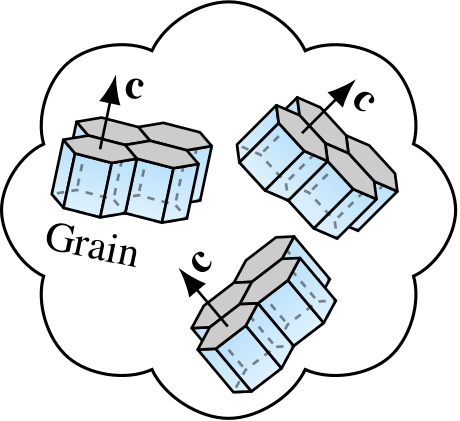
\includegraphics[scale=0.6]{../tranisotropic/polycrystal-ice.png}};

\node[] at ({-1*\dx},0*\dy) {\includegraphics[scale=1]{nlm.png}};
\node[] at ({-0.5*\dx},-0.5) {\fontsize{\fs}{\fs}\selectfont $\bf =$};

\node[] at ({0*\dx},0) {\includegraphics[scale=1]{Y00.png}};

\node[] at ({1*\dx},0) {\includegraphics[scale=1]{Y20.png}};
\node[] at ({2*\dx},0) {\includegraphics[scale=1]{Y21.png}};
\node[] at ({3*\dx},0) {\includegraphics[scale=1]{Y22.png}};

\gdef\jj{0}
\node[] at ({(\jj+0)*\dx},-\dy) {\includegraphics[scale=1]{Y40.png}};
\node[] at ({(\jj+1)*\dx},-\dy) {\includegraphics[scale=1]{Y41.png}};
\node[] at ({(\jj+2)*\dx},-\dy) {\includegraphics[scale=1]{Y42.png}};
\node[] at ({(\jj+3)*\dx},-\dy) {\includegraphics[scale=1]{Y43.png}};
\node[] at ({(\jj+4)*\dx},-\dy) {\includegraphics[scale=1]{Y44.png}};

\foreach \i in {0,...,2}
{
	\node[] at ({(\i+0.5)*\dx},-0.5) {\fontsize{\fs}{\fs}\selectfont $\bf +$};
}

\foreach \i in {-1,...,3}
{
	\node[] at ({(\i+0.5+\jj)*\dx},-0.5-\dy) {\fontsize{\fs}{\fs}\selectfont $\bf +$};
}

\end{tikzpicture}

\end{document}